\section{Illustrative Scenario}\label{sec:scenarios}
We illustrate an application of \framework\ in a realistic scenario for New York taxi dataset\footnote{\it https://data.cityofnewyork.us/view/gn7m-em8n} \cite{ferreira2013visual,FreireCVZ16}. The dataset contains 18 attributes such as pickup/dropoff date/time, passenger count and trip distance and 173,179,759 rows about taxi trips. The dataset size is 27.9 GB with informations of trips from 2014.  The following scenario illustrates how an analyst can achieve an exploratory analysis goal. We employ {\sc Highlighter} (Algorithm \ref{algo:geoh}) with following parameters: $\sigma = 0.2$, $k = 5$ and $tlimit = 200ms$. We prepared the original dataset for the running scenario and we considered a maximum of  100K unique points in our analysis. 

\begin{figure}
  \centering
  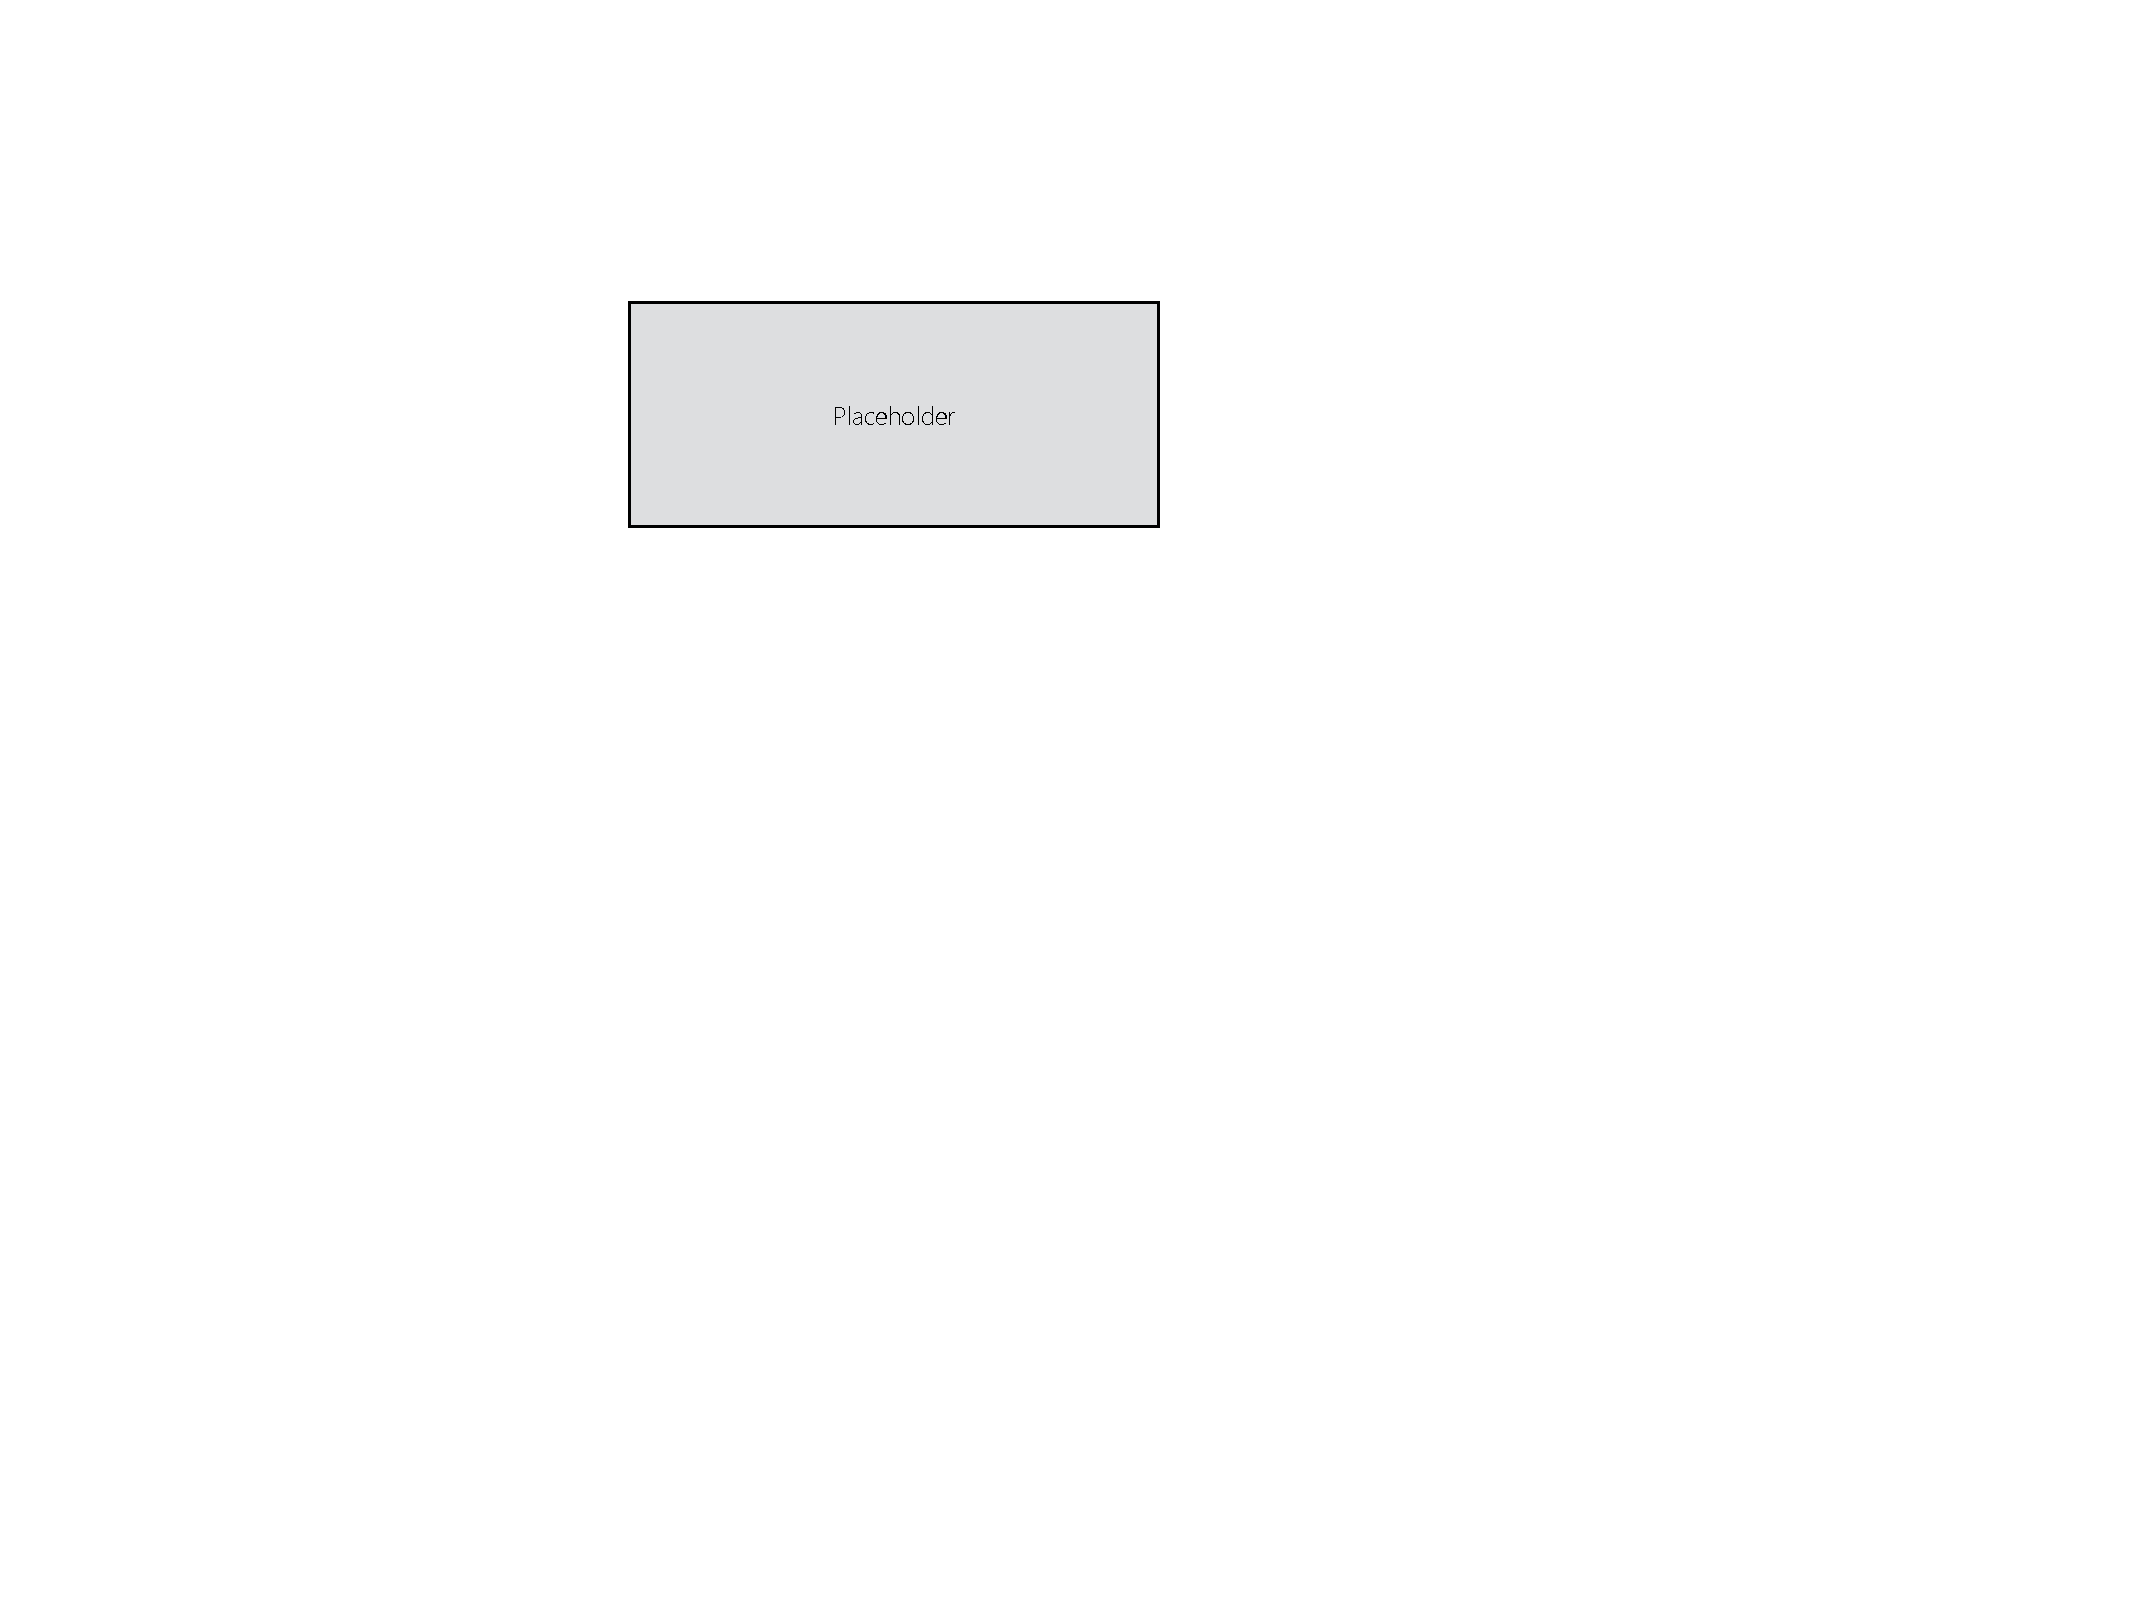
\includegraphics[width=\columnwidth]{figs/placeholder}
\caption{Application of \framework\ on New York Taxi dataset}
\label{fig:app}
\end{figure}

\vspace{5pt}
Consider Lucas, a data scientist whose task is to optimize New York taxi trips. Focusing on cab-idle locations, he wants to discover which neighborhoods work the best for which drivers to increase the overall availability. Also, he wants to discover how next cab-idle stations should be chosen to contribute to the goal. Lucas employs \framework\ and follows a case-by-case inspection as his analysis methodology.

He begins the analysis by selecting a point from the most crowded region, i.e., Times Square. The selected point depicts a drop-off\footnote{\textit{lat, long: 40.757555, -73.988832. Point ID-1274, equivalent to 270 W 43rd St, New York, NY 10036, EUA. Next to Times Square.}} around \textit{10 p.m. in January 09}.  {\sc Highlighter} then provides $5$ relevant points to the selected point (Figure \ref{fig:app}). These highlights show similar points to the selection in other neighborhoods of the region. Among 5 highlighted points, Lucas then selects the 3rd one, a pick-up\footnote{\textit{lat, long: 40.789358,-73.970172000000005. Point ID-968, equivalent to Columbus Avenue, New York, NY, EUA.}} next to \textit{ Central Park West},  at the same night because it was the nearest point at that time with a great possibility to pick-up a new passenger for a bigger distance. 

Then in the next step, {\sc Highlighter} shows 5 other points relevant to the new selection. This new result explains how drop-offs relate to neighbour locations and how next cab-idle stop can be chosen. Lucas selects the second highlighted point\footnote{\textit{lat, long: 40.717531999999999,-74.010260000000002. Point ID-192, equivalent to 183 Duane Street, New York, NY 10013, EUA}}, because of the time and distance. The other points suggested by the algorithm were next to the airport, and for that time, would be better to Lucas stay in Manhattan island and work until 1 p.m. of the next day. 

The result of similarity for all two executions of the algorithm for the Lucas problem, considering $k = 5$ and $\sigma = 0.2$, was approximately, \textit{0.72}.